\ifx\wholebook\relax \else
% ------------------------

\documentclass[b5paper]{article}
\usepackage[nomarginpar
  %, margin=.5in
]{geometry}

\addtolength{\oddsidemargin}{-0.05in}
\addtolength{\evensidemargin}{-0.05in}
\addtolength{\textwidth}{0.1in}

\usepackage[en]{../../prelude}

\setcounter{page}{1}

\begin{document}

\title{Insertion sort}

\author{Xinyu LIU
\thanks{{\bfseries Xinyu LIU} \newline
  Email: liuxinyu95@gmail.com \newline}
  }

\maketitle
\fi

\markboth{Insertion sort}{Elementary Algorithms}

\ifx\wholebook\relax
\chapter{Insertion sort}
\numberwithin{Exercise}{chapter}
\fi

\section{Introduction}
\label{sec:isort-introduction} \index{insertion sort}

Insertion sort is a straightforward sort algorithm\footnote{We skip the `Bubble sort' method\cite{wiki-bubble-sort}.}. We give its preliminary definition in chapter 1. For a collection of comparable elements, we repeatedly pick one, insert them to a list and maintain the ordering. As every insertion takes linear time, its performance is bound to $O(n)$ where $n$ is the number of elements. This performance is not as good as the divide and conqueror sort algorithms, like quick sort and merge sort. However, we can still find its application today. For example, a well tuned quick sort implementation falls back to insertion sort for small data set. The idea of insertion sort is as same as sorting a deck of a poker cards\cite{CLRS}. The cards are shuffled. A player takes card one by one. At any time, all cards on hand are sorted. When gets a new card, the player inserts it in proper position according to the order of points as shown in figure \ref{fig:hand-of-cards}.

\begin{figure}[htbp]
  \centering
  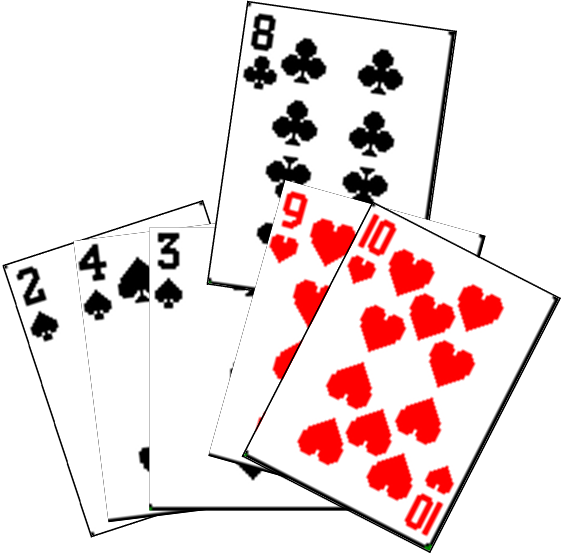
\includegraphics[scale=0.5]{img/card-deck.png}
  \caption{Insert card 8 to a deck.}
  \label{fig:hand-of-cards}
\end{figure}

Based on this idea, we can implement insertion sort as below:

\begin{algorithmic}
\Function{Sort}{$A$}
  \State $X \gets \phi$
  \For{each $x \in A$}
    \State \Call{Insert}{$X, x$}
  \EndFor
  \State \Return $X$
\EndFunction
\end{algorithmic}

It's easy to express this process with folding, which we
mentioned in the chapter of binary search tree.

\be
  sort = foldL \quad insert \quad \phi
\ee

Note that in the above algorithm, we store the sorted result in $X$,
so this isn't in-place sorting. It's easy to change it to in-place
algorithm. Denote the sequence as $A = \{a_1, a_2, ..., a_n\}$.

\begin{algorithmic}
\Function{Sort}{$A$}
  \For{$i \gets 2$ to $|A|$}
    \State insert $a_i$ to sorted sequence $\{a'_1, a'_2, ..., a'_{i-1} \}$
  \EndFor
\EndFunction
\end{algorithmic}

At any time, when we process the $i$-th element, all elements before $i$
have already been sorted. we continuously insert the current elements
until consume all the unsorted data. This idea is illustrated as in figure
\ref{fig:in-place-sort}.

\begin{figure}[htbp]
  \centering
  \includegraphics[scale=0.8]{img/in-place-sort.ps}
  \caption{The left part is sorted data, continuously insert elements to sorted part.}
  \label{fig:in-place-sort}
\end{figure}

We can find there is recursive concept in this definition. Thus it can
be expressed as the following.

\be
sort(A) = \left \{
  \begin{array}
  {r@{\quad:\quad}l}
  \phi & A = \phi \\
  insert(sort(\{a_2, a_3, ...\}), a_1) & otherwise
  \end{array}
\right.
\ee

% ================================================================
% Insertion
% ================================================================
\section{Insertion}
\index{insertion sort!insertion}

We haven't answered the question about how to realize insertion however.
It's a puzzle how does human locate the proper position so quickly.

For computer, it's an obvious option to perform a scan. We can either
scan from left to right or vice versa. However, if the sequence is
stored in plain array, it's necessary to scan from right to left.

\begin{algorithmic}
\Function{Sort}{$A$}
  \For{$i \gets 2$ to $|A|$}
    \Comment{Insert $A[i]$ to sorted sequence $A[1...i-1]$}
    \State $x \gets A[i]$
    \State $j \gets i-1$
    \While{$j > 0 \land x < A[j]$ }
      \State $A[j+1] \gets A[j]$
      \State $j \gets j - 1$
    \EndWhile
    \State $A[j+1] \gets x$
  \EndFor
\EndFunction
\end{algorithmic}

One may think scan from left to right is natural. However, it isn't
as effect as above algorithm for plain array. The reason is that, it's
expensive to insert an element in arbitrary position in an array.
As array stores elements continuously, if we want to insert new element
$x$ in position $i$, we must shift all elements after $i$, including
$i+1, i+2, ...$ one position to right. After that the cell at position $i$
is empty, and we can put $x$ in it. This is illustrated in
figure \ref{fig:array-shift}.

\begin{figure}[htbp]
  \centering
  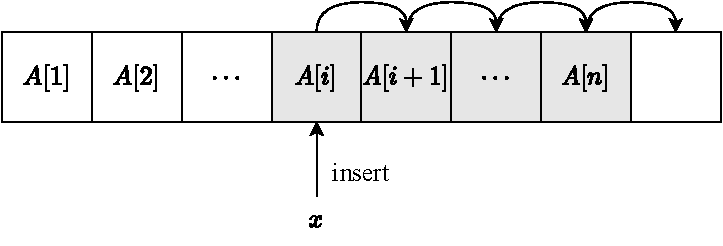
\includegraphics[scale=0.7]{img/array-shift.ps}
  \caption{Insert $x$ to array $A$ at position $i$.}
  \label{fig:array-shift}
\end{figure}

If the length of array is $n$, this indicates we need examine the
first $i$ elements, then perform
$n-i+1$ moves, and then insert $x$ to the $i$-th cell. So insertion
from left to right need traverse the whole array anyway.
While if we scan from right to
left, we examine $i$ elements at most, and perform the same
amount of moves.

Translate the above algorithm to Python yields the following code.

\lstset{language=Python}
\begin{lstlisting}
def isort(xs):
    n = len(xs)
    for i in range(1, n):
        x = xs[i]
        j = i - 1
        while j >= 0 and x < xs[j]:
            xs[j+1] = xs[j]
            j = j - 1
        xs[j+1] = x
\end{lstlisting}

It can be found some other equivalent programs, for instance the following
ANSI C program. However this version isn't as effective as the pseudo code.

\lstset{language=C}
\begin{lstlisting}
void isort(Key* xs, int n){
  int i, j;
  for(i=1; i<n; ++i)
    for(j=i-1; j>=0 && xs[j+1] < xs[j]; --j)
      swap(xs, j, j+1);
}
\end{lstlisting}

This is because the swapping function, which can exchange two elements
typically uses a temporary variable like the following:

\begin{lstlisting}
void swap(Key* xs, int i, int j){
  Key temp = xs[i];
  xs[i] = xs[j];
  xs[j] = temp;
}
\end{lstlisting}

So the ANSI C program presented above takes $3m$ times assignment, where $m$
is the number of inner loops. While the pseudo code as well as the Python
program use shift operation instead of swapping. There are $m+2$ times
assignment.

We can also provide \textproc{Insert}() function explicitly, and call it
from the general insertion sort algorithm in previous section. We skip
the detailed realization here and left it as an exercise.

All the insertion algorithms are bound to $O(n)$, where $n$ is the length of
the sequence. No matter what difference among them, such as scan from left
or from right. Thus the over all performance for insertion sort is quadratic
as $O(n^2)$.

\begin{Exercise}

\begin{itemize}
\item Provide explicit insertion function, and call it with general
insertion sort algorithm. Please realize it in both procedural way and
functional way.
\end{itemize}

\end{Exercise}

% ================================================================
% Improvement 1
% ================================================================

\section{Improvement 1}
\index{Insertion sort!binary search}

Let's go back to the question, that why human being can find the proper
position for insertion so quickly. We have shown a solution based on scan.
Note the fact that at any time, all cards at hands have been well sorted,
another possible solution is to use binary search to find that location.

We'll explain the search algorithms in other dedicated chapter. Binary
search is just briefly introduced for illustration purpose here.

The algorithm will be changed to call a binary search procedure.

\begin{algorithmic}
\Function{Sort}{$A$}
  \For{$i \gets 2$ to $|A|$}
    \State $x \gets A[i]$
    \State $p \gets $ \Call{Binary-Search}{$A[1...i-1], x$}
    \For{$j \gets i$ down to $p$}
      \State $A[j] \gets A[j-1]$
    \EndFor
    \State $A[p] \gets x$
  \EndFor
\EndFunction
\end{algorithmic}

Instead of scan elements one by one, binary search utilize the information
that all elements in slice of array $\{A_1, ..., A_{i-1} \}$ are sorted.
Let's assume
the order is monotonic increase order. To find a position $j$ that satisfies
$A_{j-1} \leq x \leq A_{j}$. We can first examine the middle element, for
example, $A_{\lfloor i/2 \rfloor}$. If $x$ is less than it, we need next recursively
perform binary search in the first half of the sequence; otherwise, we
only need search in last half.

Every time, we halve the elements to be examined, this search process runs
$O(\lg n)$ time to locate the insertion position.

\begin{algorithmic}
\Function{Binary-Search}{$A, x$}
  \State $l \gets 1$
  \State $u \gets 1+|A|$
  \While{$l < u$}
    \State $m \gets \lfloor \frac{l+u}{2} \rfloor$
    \If{$A[m] = x$}
      \State \Return $m$ \Comment{Find a duplicated element}
    \ElsIf{$A[m] < x$}
      \State $l \gets m+1$
    \Else
      \State $u \gets m$
    \EndIf
  \EndWhile
  \State \Return $l$
\EndFunction
\end{algorithmic}

The improved insertion sort algorithm is still bound to $O(n^2)$,
compare to previous section, which we use $O(n^2)$ times comparison and
$O(n^2)$ moves, with binary search, we just use $O(n \lg n)$ times
comparison and $O(n^2)$ moves.

The Python program regarding to this algorithm is given below.

\lstset{language=Python}
\begin{lstlisting}
def isort(xs):
    n = len(xs)
    for i in range(1, n):
        x = xs[i]
        p = binary_search(xs[:i], x)
        for j in range(i, p, -1):
            xs[j] = xs[j-1]
        xs[p] = x

def binary_search(xs, x):
    l = 0
    u = len(xs)
    while l < u:
        m = (l+u)/2
        if xs[m] == x:
            return m
        elif xs[m] < x:
            l = m + 1
        else:
            u = m
    return l
\end{lstlisting}

\begin{Exercise}
Write the binary search in recursive manner. You needn't use purely functional
programming language.
\end{Exercise}

% ================================================================
% Improvement 2
% ================================================================

\section{Improvement 2}
\index{Insertion sort!linked-list setting}

Although we improve the search time to $O(n \lg n)$ in previous section, the
number of moves is still $O(n^2)$. The reason of why movement takes so long
time, is because the sequence is stored in plain array. The nature of array
is continuously layout data structure, so the insertion operation is expensive.
This hints us that we can use linked-list setting to represent the sequence.
It can improve the insertion operation from $O(n)$ to constant time $O(1)$.

\be
  insert(A, x) = \left \{
  \begin{array}
  {r@{\quad:\quad}l}
  \{ x \} & A = \phi \\
  \{ x \} \cup A & x < a_1 \\
  \{ a_1 \} \cup insert(\{ a_2, a_3, ... a_n\}, x)& otherwise
  \end{array}
\right.
\ee

Translating the algorithm to Haskell yields the below program.

\lstset{language=Haskell}
\begin{lstlisting}
insert [] x = [x]
insert (y:ys) x = if x < y then x:y:ys else y:insert ys x
\end{lstlisting}

And we can complete the two versions of insertion sort program based on
the first two equations in this chapter.

\begin{lstlisting}
isort [] = []
isort (x:xs) = insert (isort xs) x
\end{lstlisting}

Or we can represent the recursion with folding.

\begin{lstlisting}
isort = foldl insert []
\end{lstlisting}

Linked-list setting solution can also be described imperatively. Suppose
function \textproc{Key}($x$), returns the value of element stored in node
$x$, and \textproc{Next}($x$) accesses the next node in the linked-list.

\begin{algorithmic}
\Function{Insert}{$L, x$}
  \State $p \gets$ NIL
  \State $H \gets L$
  \While{$L \neq$ NIL $\land $ \Call{Key}{$L$} $<$ \Call{Key}{$x$}}
    \State $p \gets L$
    \State $L \gets $ \Call{Next}{$L$}
  \EndWhile
  \State \Call{Next}{$x$} $\gets L$
  \If{$p =$ NIL}
    \State $H \gets x$
  \Else
    \State \Call{Next}{$p$} $\gets x$
  \EndIf
  \State \Return $H$
\EndFunction
\end{algorithmic}

For example in ANSI C, the linked-list can be defined as the following.

\lstset{language=C}
\begin{lstlisting}
struct node{
  Key key;
  struct node* next;
};
\end{lstlisting}

Thus the insert function can be given as below.

\begin{lstlisting}
struct node* insert(struct node* lst, struct node* x){
  struct node *p, *head;
  p = NULL;
  for(head = lst; lst && x->key > lst->key; lst = lst->next)
    p = lst;
  x->next = lst;
  if(!p)
    return x;
  p->next = x;
  return head;
}
\end{lstlisting}

Instead of using explicit linked-list such as by pointer or reference
based structure. Linked-list can also be realized by another index array.
For any array element $A[i]$, $Next[i]$ stores the index of next element
follows $A[i]$. It means $A[Next[i]]$ is the next element after $A[i]$.

The insertion algorithm based on this solution is given like below.

\begin{algorithmic}
\Function{Insert}{$A, Next, i$}
  \State $j \gets \perp$
  \While{$Next[j] \neq$ NIL $\land A[Next[j]] < A[i]$}
    \State $j \gets Next[j]$
  \EndWhile
  \State $Next[i] \gets Next[j]$
  \State $Next[j] \gets i$
\EndFunction
\end{algorithmic}

Here $\perp$ means the head of the $Next$ table.
And the relative Python program for this algorithm is given as the following.

\lstset{language=Python}
\begin{lstlisting}
def isort(xs):
    n = len(xs)
    next = [-1]*(n+1)
    for i in range(n):
        insert(xs, next, i)
    return next

def insert(xs, next, i):
    j = -1
    while next[j] != -1 and xs[next[j]] < xs[i]:
        j = next[j]
    next[j], next[i] = i, next[j]
\end{lstlisting}

Although we change the insertion operation to constant time by using
linked-list. However, we have to traverse the linked-list to find the
position, which results $O(n^2)$ times comparison. This is because
linked-list, unlike array, doesn't support random access. It means we
can't use binary search with linked-list setting.

\begin{Exercise}
\begin{itemize}
\item Complete the insertion sort by using linked-list insertion function
in your favorate imperative programming language.
\item The index based linked-list return the sequence of rearranged index
as result. Write a program to re-order the original array of elements from
this result.
\end{itemize}
\end{Exercise}

% ================================================================
% Final improvement
% ================================================================

\section{Final improvement by binary search tree}
\index{Insertion sort!binary search tree}

It seems that we drive into a corner. We must improve both the comparison
and the insertion at the same time, or we will end up with $O(n^2)$ performance.

We must use binary search, this is the only way to improve the comparison
time to $O(\lg n)$. On the other hand, we must change the data structure,
because we can't achieve constant time insertion at a position with
plain array.

This remind us about our 'hello world' data structure, binary search tree.
It naturally support binary search from its definition. At the same time,
We can insert a new node in binary search tree in $O(1)$ constant time
if we already find the location.

So the algorithm changes to this.

\begin{algorithmic}
\Function{Sort}{$A$}
  \State $T \gets \phi$
  \For{each $x \in A$}
    \State $T \gets $ \Call{Insert-Tree}{$T, x$}
  \EndFor
  \State \Return \Call{To-List}{$T$}
\EndFunction
\end{algorithmic}

Where \textproc{Insert-Tree}() and \textproc{To-List}() are described in
previous chapter about binary search tree.

As we have analyzed for binary search tree, the performance of tree sort
is bound to $O(n \lg n)$, which is the lower limit of comparison based
sort\cite{Knuth}.

\section{Short summary}
In this chapter, we present the evolution process of insertion sort. Insertion
sort is well explained in most textbooks as the first sorting algorithm.
It has simple and straightforward idea, but the performance is quadratic.
Some textbooks stop here, but we want to show that there exist ways to improve
it by different point of view. We first try to save the comparison time
by using binary search, and then try to save the insertion operation by
changing the data structure to linked-list. Finally, we combine these
two ideas and evolute insertion sort to tree sort.

\begin{thebibliography}{99}

\bibitem{wiki-bubble-sort}
http://en.wikipedia.org/wiki/Bubble\_sort

\bibitem{CLRS}
Thomas H. Cormen, Charles E. Leiserson, Ronald L. Rivest and Clifford Stein.
``Introduction to Algorithms, Second Edition''. ISBN:0262032937. The MIT Press. 2001

\bibitem{Knuth}
Donald E. Knuth. ``The Art of Computer Programming, Volume 3: Sorting and Searching (2nd Edition)''. Addison-Wesley Professional; 2 edition (May 4, 1998) ISBN-10: 0201896850 ISBN-13: 978-0201896855

\end{thebibliography}

\ifx\wholebook\relax\else
\end{document}
\fi
